\section{Question}

\subsection{Now consider the phylogenetic implications of your results. First, create a BLAST tree (using the function 'Distance tree of results').}

\begin{figure}[ht]
    \centering
    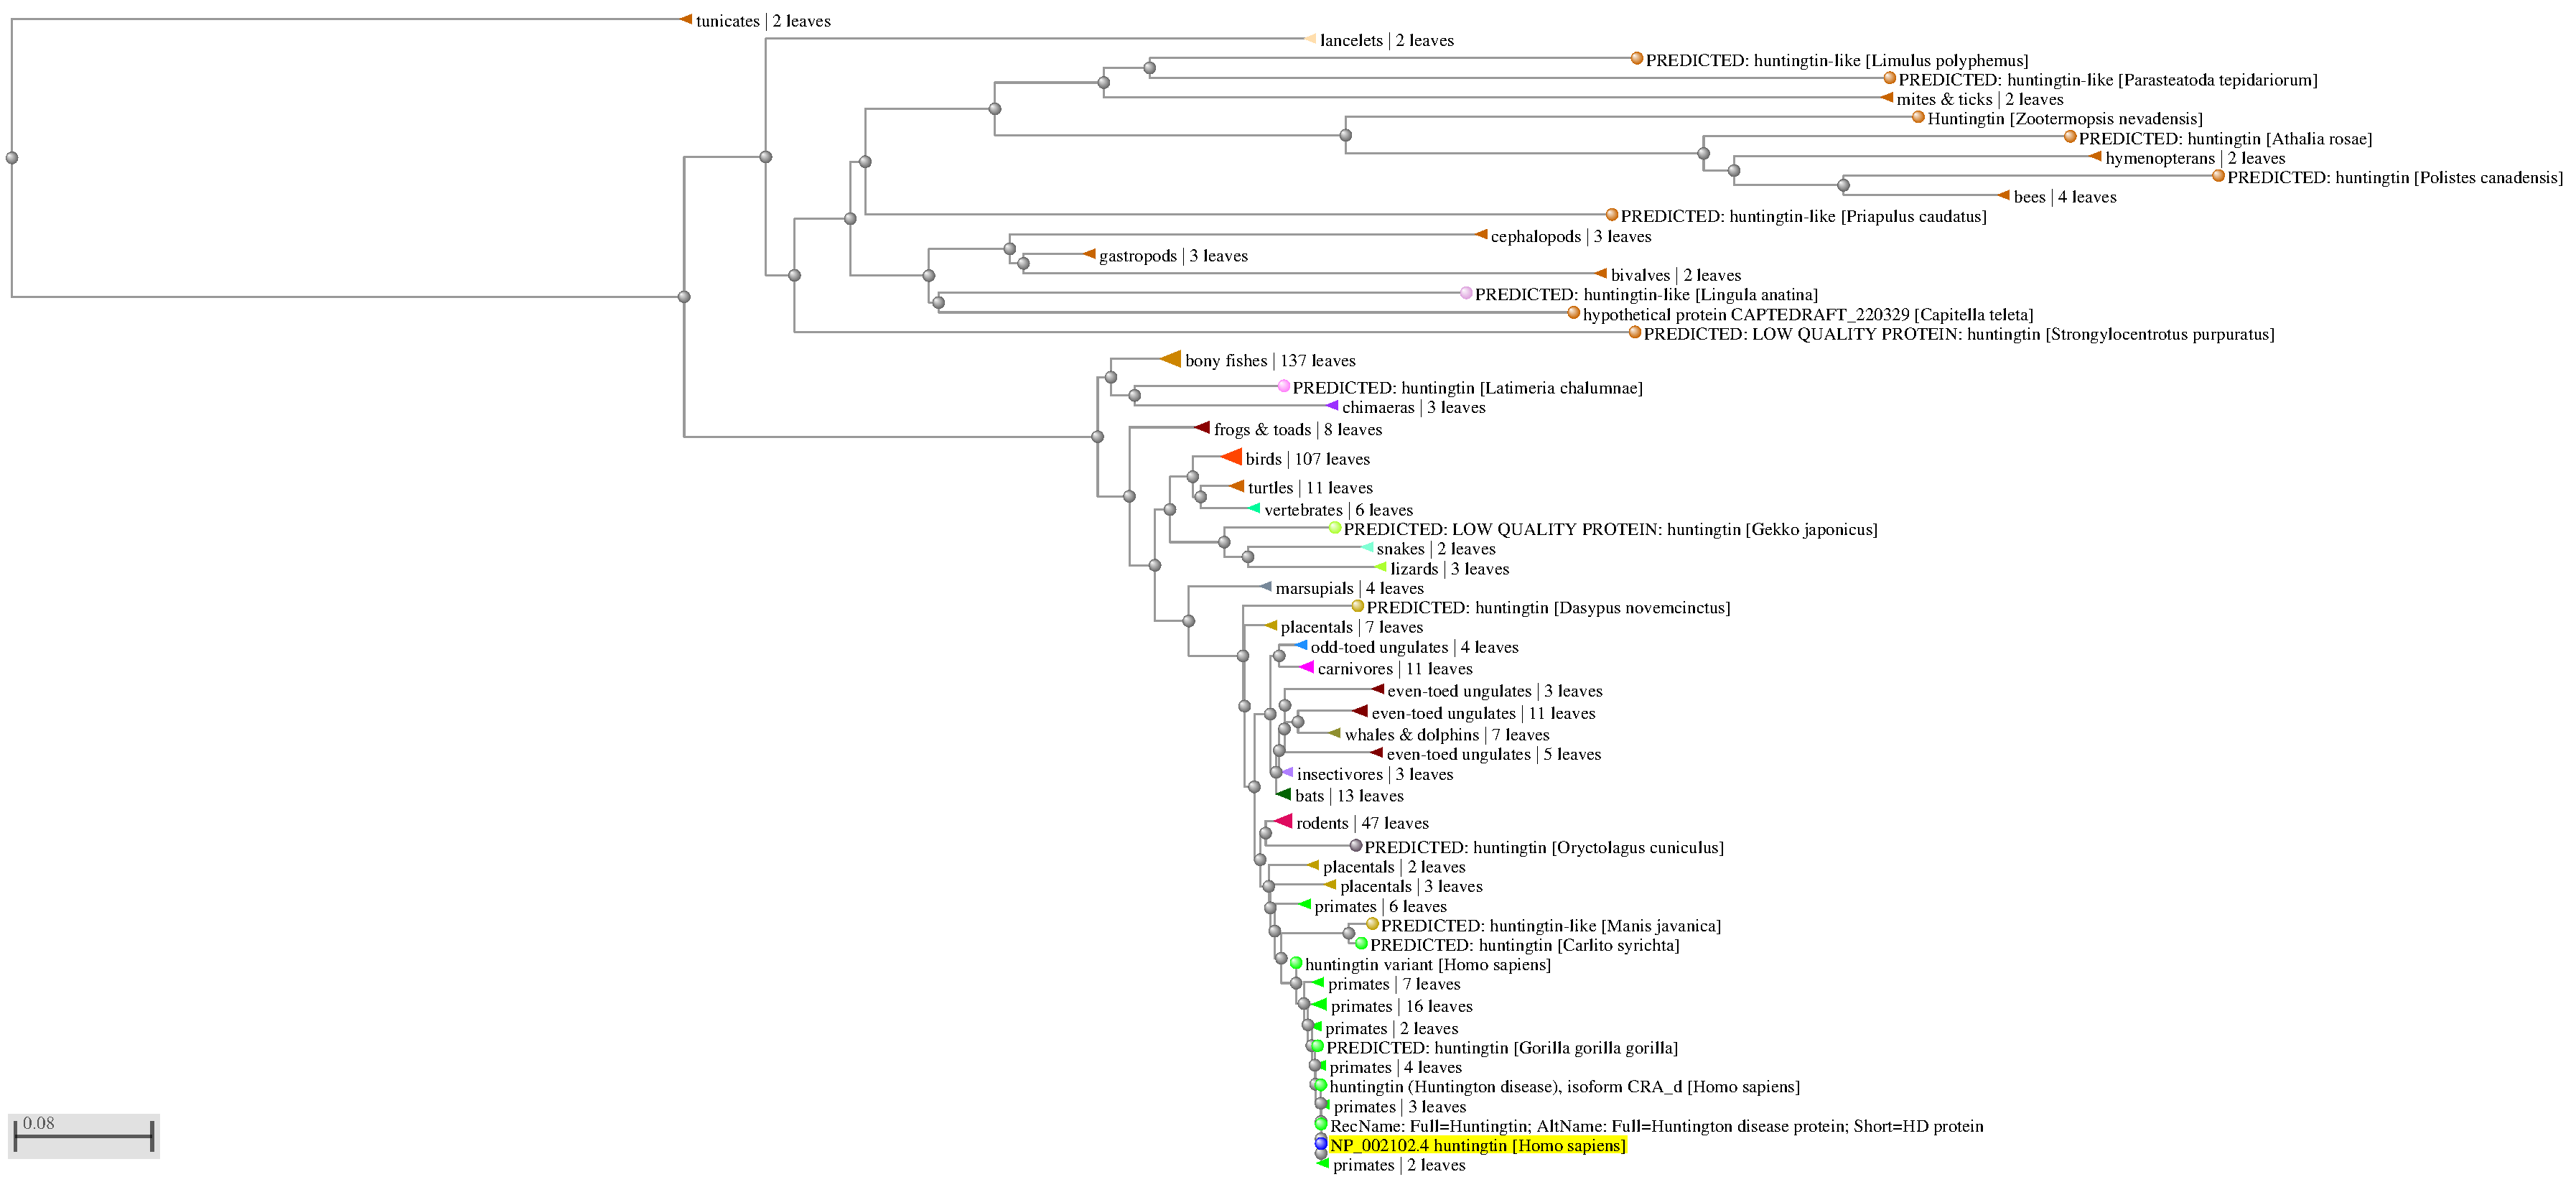
\includegraphics[width=\linewidth]{res/blast-tree.pdf}
    \caption{Distance tree generated from the BLAST query.}
    \label{fig:blast-tree}
\end{figure}

% - - - - - - - - - - - - - - - - - - - - - - - - - - -

\subsection{Describe the result and its relevance.}

The resulting distance tree is a visual representation of the relationship between organisms related to the \textit{huntingtin} gene and their ancestors.

It is relevant to analyse and study the proximity of organisms which express the same gene one is researching - \textit{huntingtin} in this case.

\begin{figure}[ht]
    \centering
    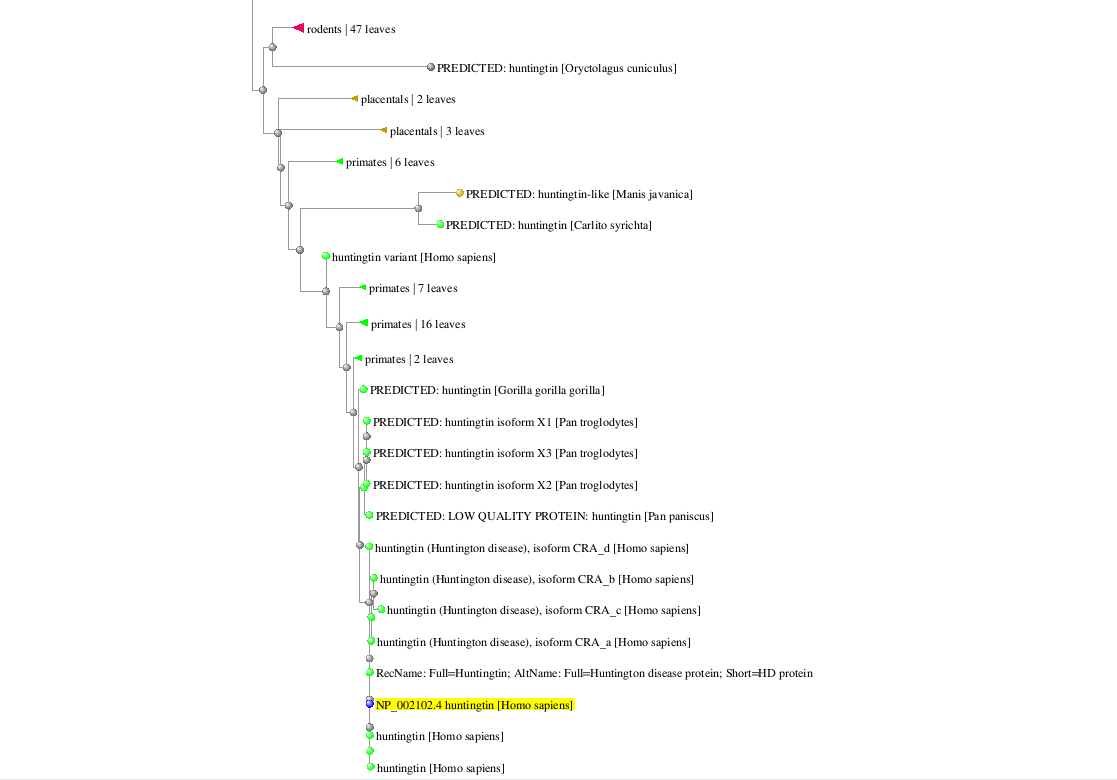
\includegraphics[width=0.7\linewidth]{res/blast-tree-zoom.png}
    \caption{Sub-tree of the distance tree in figure \ref{fig:blast-tree}.}
    \label{fig:blast-subtree}
\end{figure}

% - - - - - - - - - - - - - - - - - - - - - - - - - - -

\subsection{How can this be used to study the disease in another model organism?}

As it has been previously said, this kind of representation - distance tree obtained with blast - can be used to list in a tree structure organisms which are closely related to the disease.

This is very useful for situations where one needs to look for a model organism to study a disease.

For example, in our case we are interested in \textit{HD}. If we wanted to use a model organism to study the disease gene expressed in humans, we would like to choose the model organism as close to humans as possible. The tree representation makes it easier to answer this question: one can look for the leaf where the gene is expressed, and from there look for the nearest leaf which corresponds to a model organism.

% - - - - - - - - - - - - - - - - - - - - - - - - - - -

\subsection{Are there known orthologues in mouse, fruit fly or yeast?}

There are for the mouse and for the fruit fly, but not for yeast. The \textit{NCBI} database contains \href{https://www.ncbi.nlm.nih.gov/gene/?Term=ortholog_gene_3064[group]}{orthologs of numerous species}, including \href{https://www.ncbi.nlm.nih.gov/gene/15194}{\textit{Mus musculus}} and \href{https://www.ncbi.nlm.nih.gov/gene/43392}{\textit{Drosophila melanogaster}}.


% - - - - - - - - - - - - - - - - - - - - - - - - - - -

\subsection{Using the information under 'General gene information', discuss whether mouse, fruit fly or yeast (or any of these for which an orthologue exists) are suitable models to study the disease.}

\textbf{Note: To give an example, if the gene is implicated in cell cycle, yeast may well be a good model because it is easier to study than mice. But if the gene is relevant for brain function, yeast may of course be less relevant even if an orthologue exists.}

From the \textit{General gene information} - \url{https://www.ncbi.nlm.nih.gov/gene/3064#general-gene-info} - one can read: \textit{The HTT gene is conserved in chimpanzee, dog, cow, mouse, rat, chicken, zebrafish, and frog.}

Considering the disease symptoms and taking into account other details discussed on Assignment 1, the mouse is the most suitable model to study the disease. Yeast is not an ortholog of the gene, and the mouse should be chosen over the fruit fly because its proximity to \textit{H. Sapiens} is much greater.

\newpage
